\documentclass[a4paper]{scrartcl}
\usepackage{wrapfig}
\usepackage{geometry}
 \geometry{
 a4paper,
 total={210mm,297mm},
 left=1in,
 right=1in,
 top=0.75in,
 bottom=0.8in,
 }
\usepackage{graphicx}
%\usepackage[T1]{fontenc}
\usepackage{todonotes}
\usepackage{hyperref}
\hypersetup{
    colorlinks=true,
    linkcolor=blue,
    filecolor=magenta,      
    urlcolor=blue,
}
\usepackage[figurename=Fig.]{caption}

\begin{document}

\title{Automated App-based Plant Disease Identification From Images Using Artifical Intelligence}
\subtitle{Sector: Agriculture}
\author{
\href{mailto:sasankchilamkurthy@gmail.com}{Sasank Chilamkurthy}, B.Tech, IIT Bombay\\
\href{mailto:prudhvitej.immadi@gmail.com}{Prudhvi Tej}, B.Tech, IIT Bombay\\
\href{mailto:preethamsreenivas@gmail.com}{Preetham Sreenivas}, B.Tech, IIT Bombay
}

\maketitle

\begin{abstract}
Plant diseases present a challenge in attaining food security and wrong diagnosis of the disease can have disastrous consequences for small-holder farmers. 
At the same time, timely diagnosis allow for a much more effective disease management and hence enhance yield of the crop.
Taking advantage of rapid uptake of smartphones in India, we propose to develop an app-based automated plant disease diagnosis system. 
Researchers were able to achieve accuracies nearing 100\% in disease identification from images.
We explain this technology and lay an actionable plan to the extend this to all the crops and diseases.


\end{abstract}

\section{Introduction}
Food security is an important concern for a developing country like India.
India has achieved self sufficiency post-independence in about two decades.
However, there has been a decline in growth rates of production and yield in the recent past (1996-08 -- 0.93\% as compared to 1986-97 -- 2.93\%). 
The growth rate of production is also much lower than that of population\cite{dev2010food}.
This is only exacerbated by number of factors like climate change\cite{tai2014threat} and plant diseases\cite{strange2005plant}.

Plant diseases are not only a threat to food security, but can also have a disastrous consequences for small-holder farmers whose livelihoods depend on healthy crops. 
In a country where overwhelming majority of farmers are small-holders\cite{ifad2013smallholders} and with higher incidence of farmer's suicides \cite{mishra2014}, 
there is a pressing need for effective plant disease management.

Identification of the plant disease as soon as possible forms a crucial step in efficient plant disease management. 
Disease identification is currently supported by network of experts hired by Department of Agriculture. 
However, there are not enough of them to diagnose all the crops in an area and
farmers have to resort to ill-trained salesmen of chemical companies for their disease diagnosis needs.
Such a situation calls for a technological intervention for plant disease identification.

\section{Challenge}
There is a rapid uptake of mobile phone technology in India. Indeed, India is now the world's second biggest smartphone market and low budget smart phones are especially popular in the farmer community.  
Novel approaches can be designed to use these phones to identify diseases using their computing power, high resolution displays, and built-in accessories such as HD cameras.

Given such wide penetration of smartphones in India, disease diagnosis based on automated image recognition can be made available at an unprecedented scale. 
This will particularly benefit small-holder farmers as they cannot bear the cost of wrongly sprayed chemicals. 

So, we frame our problem as follows:  
\begin{center}
\framebox{Given an image of a plant leaf, develop an application to identify the disease of the plant automatically}
\end{center}
It can also be used as an effective tool to disseminate information about latest agricultural practices to farming community. Once a plant disease is diagnosed, it can be followed up with current best practices to manage that particular plant disease. 

\section{Technological Solution}

Artificial intelligence (AI), computer vision, and object recognition in particular, has made tremendous advances in the past few years. In 2015, a large, deep convolutional neural network achieved a top-5 error of 3.57\% for the classification of images into 1,000 possible categories\cite{DBLP:journals/corr/HeZRS15}.
These images are taken from the web and represent the variability of real world images.

In order to develop accurate image classifiers for the purposes of plant disease diagnosis, we need a large, verified dataset of images of diseased and healthy plants. Until very recently, such a data set did not exist, and even smaller datasets were not freely available. To address this problem, a project called PlantVillage has begun collecting tens of thousands of images of healthy and diseased crop plants \cite{hughes2015open, mohanty2016inference}

This dataset has 54,306 images of 26 diseases in 14 crop species. 
A preprint published in as recent as April 2016 already reports 99\% accuracy on this dataset\cite{mohanty2016inference}.
A sample of images from the dataset are shown in figure \ref{fig:leaf}.


\begin{figure}[ht]
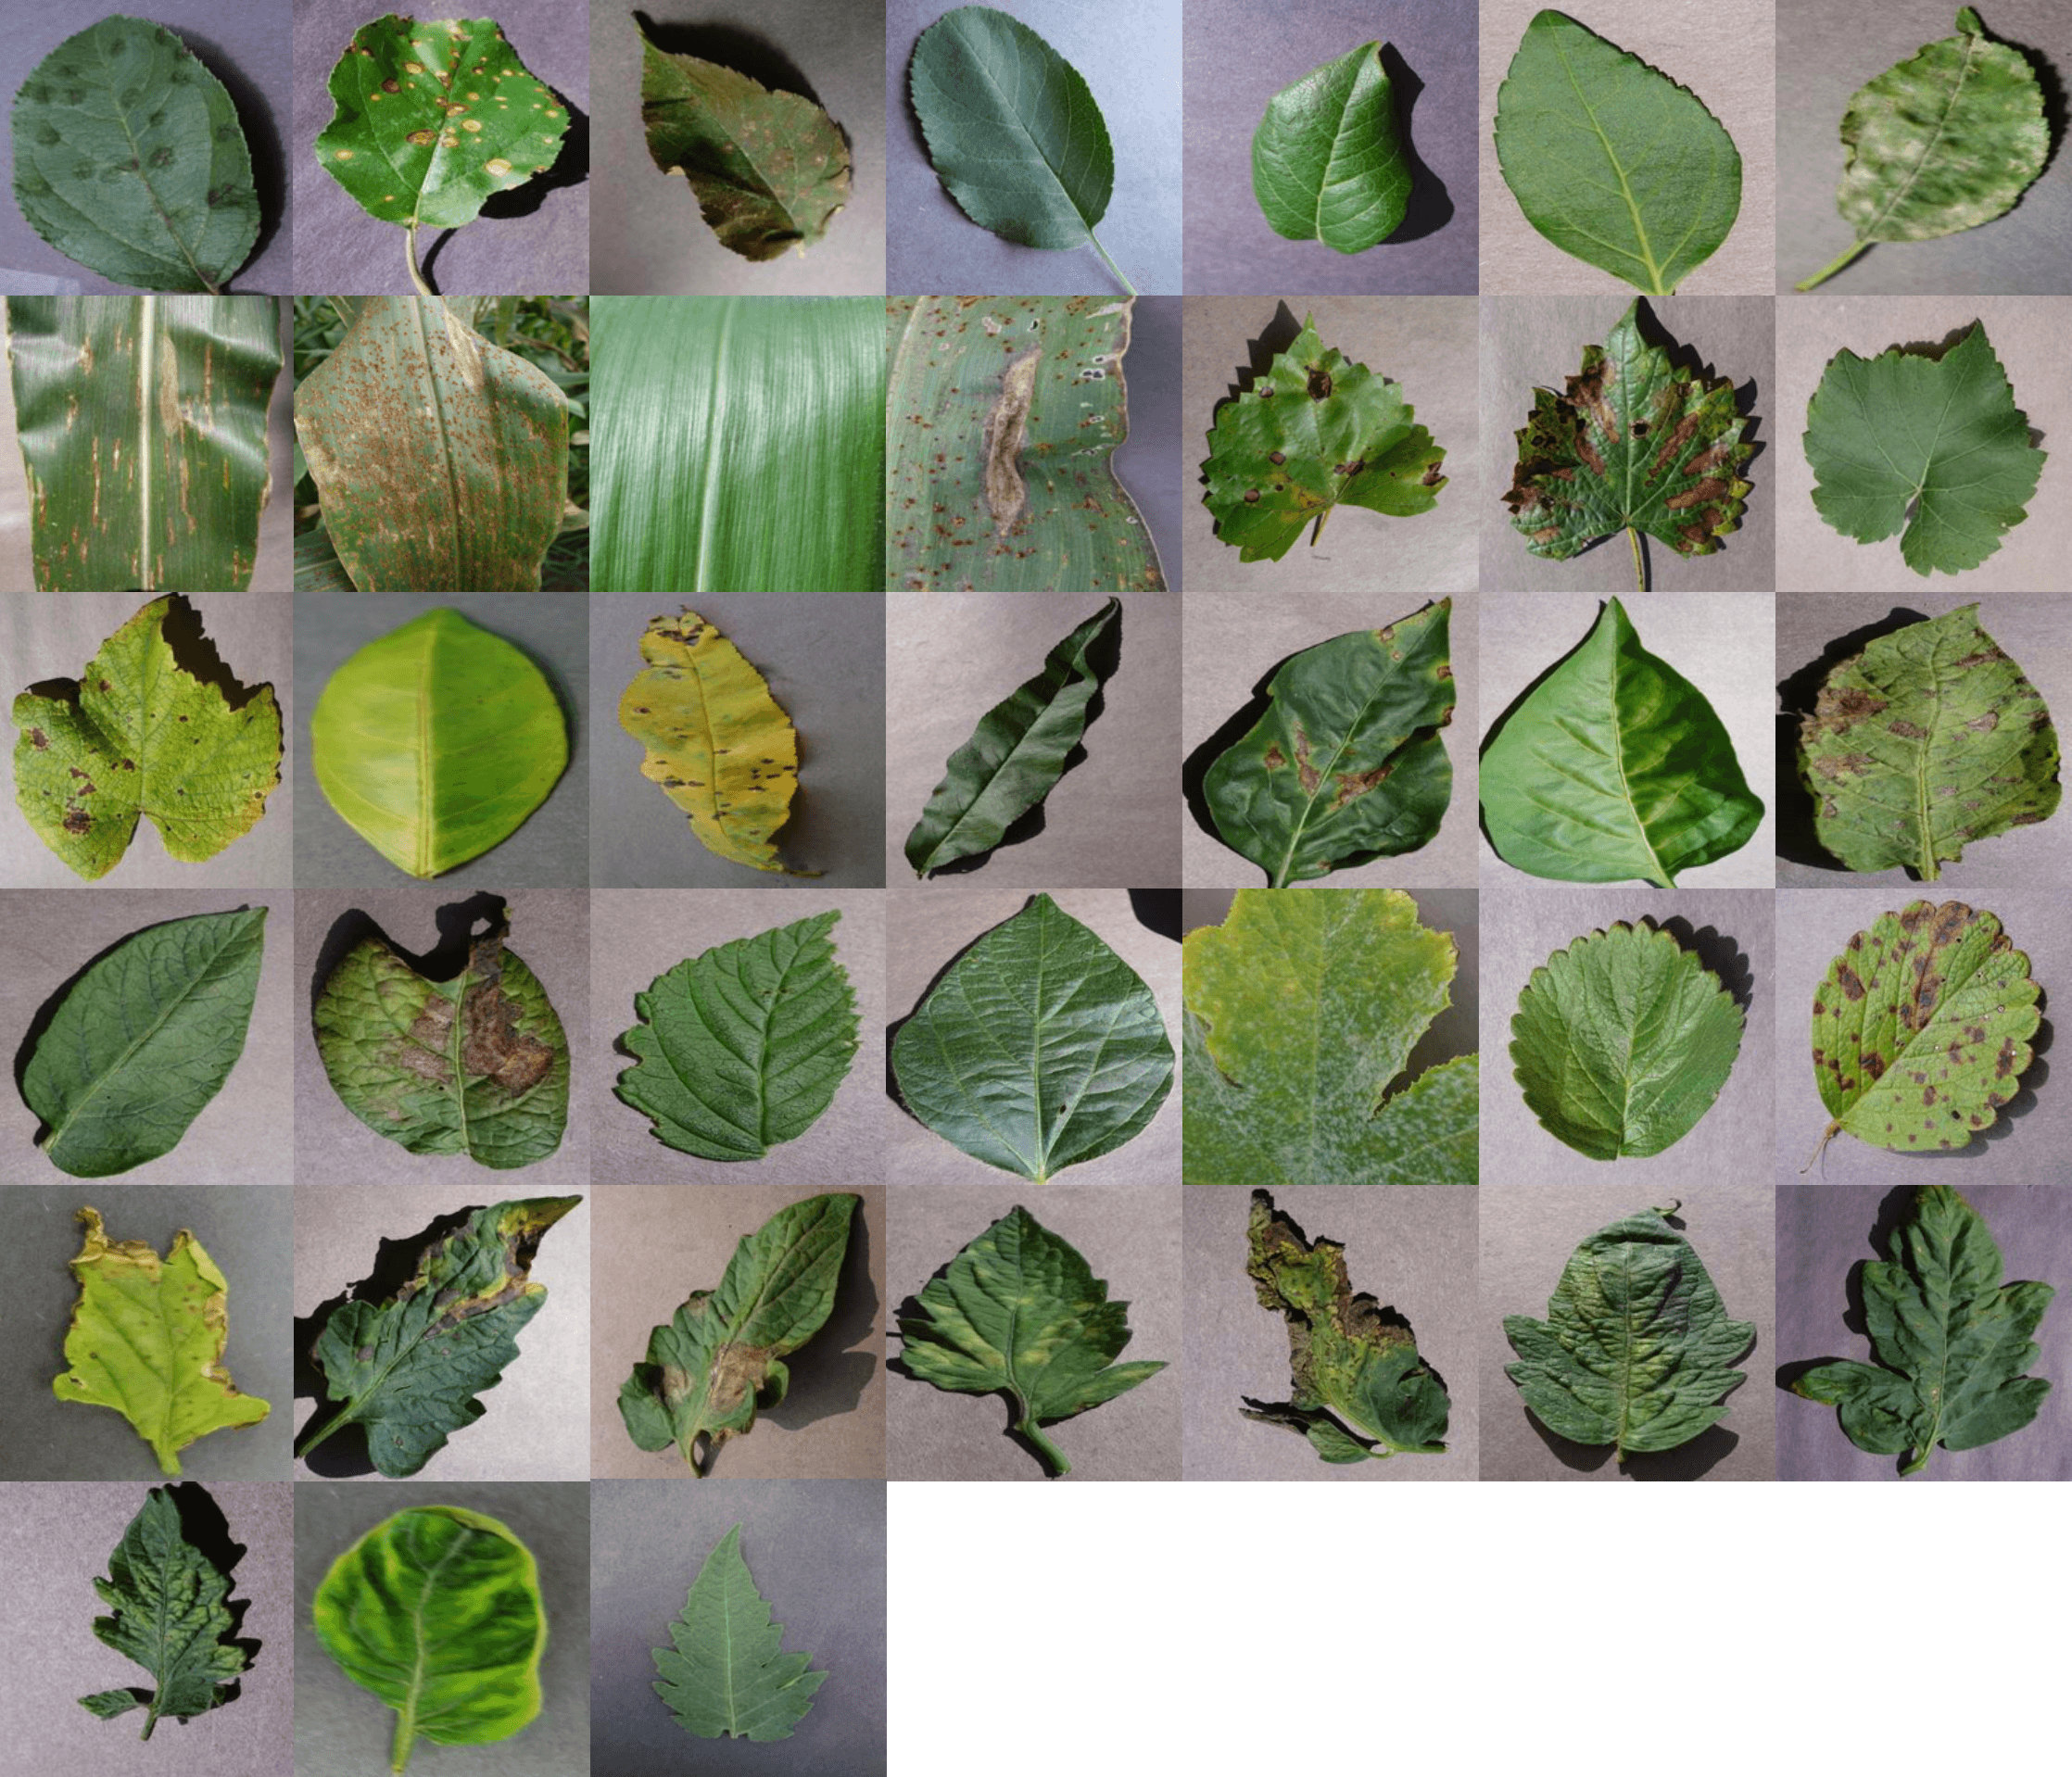
\includegraphics[width=14cm]{plantvillage-min.png}
\centering
\caption{38 Classes of PlantVillage dataset}
\label{fig:leaf}
\end{figure}

\section{Discussion}
As can be seen in figure \ref{fig:leaf}, PlantVillage dataset covers neither all the crops nor all the diseases for a given crop. 
However, if a dataset of this scale can be made for each crop which covers all of its diseases, disease diagnosis by an automated algorithm will almost be perfect. 
With resources a governmental department has and the tremendous promise of the approach, procuring such a dataset of images should not be difficult.

\subsection{Conclusion}
Given the urgency of improving yield and importance of modernisation of agriculture in Indian context, we think solving the problem of information asymmetry between farmers and agricultural researchers is vital to the sustainability of Indian agriculture. 
We also provide technology and an actionable plan to solve the problem.

\bibliography{nitiaayog}
\bibliographystyle{acm}

\end{document}